\documentclass[a4paper]{article}
\usepackage{graphicx}
\usepackage{indentfirst}
\usepackage{fancyhdr}
\usepackage{url}
\usepackage[colorlinks=true,linkcolor=blue,filecolor=blue,urlcolor=blue]{hyperref}
\usepackage[top=30truemm,bottom=30truemm,left=25truemm,right=25truemm]{geometry}

\pagestyle{fancy}
\fancyhf{}
\rhead{\thepage}
\lhead{PFS Operational Plan}
\rfoot{}

\title{Subaru Prime Focus Spectrograph (PFS) Operational Plan}
\author{Kiyoto Yabe (Kavli IPMU)}
%%\date{}

\begin{document}
\maketitle
\tableofcontents

\clearpage
%%%%%%%%%%%
%% Background %%
%%%%%%%%%%%
\section{Background}
PFS is an open use instrument of the Subaru Telescope starting its
commissioning from 2018 and the scientific operation from 2019. In
this document, we describe the operation concept of PFS system during
the commissioning phase and after the scientific operation starts. One
of the aims of writing this document is not only to define the overall
concept of the operation but also to check the possibility of the
discontinuity between the operational concept and the telescope system
in the Subaru Telescope (including Gen2 and archival system such as
STARS/MSTARS) through conversations between the observatory and the
PFS project team to mitigate the risk after the commissioning
starts. Therefore, some descriptions in this document is of course
subject to be updated in the future.

\section{PFS System Description\label{sec:pfs_system}}
Here, we briefly summarize PFS instrument system, which is described
in the technical documents in more detail(e.g. \cite{tamura16}).

PFS is a fiber-fed type spectrograph mounted on the prime focus of the
Subaru Telescope. The distinctive features are a wide area of FoV of
$\sim1.3$ deg$^{2}$, a large multiplicity of $\sim2400$ fibers, and a
wide range of wavelength coverage from 380 nm to 1260 nm. PFS
comprises several instruments: Prime Focus Instrument (PFI), Fiber
system, Spectrograph System (SpS), and Metrology Camera System
(MCS). These components are driven independently and sparsely
connected in software controlled on the Messaging Hub System (MHS). In
the following subsections, a brief summary of each component is
described.

\subsection{Prime Focus Instrument (PFI)\label{sec:pfs_system:pfi}}
At the Subaru prime focus, HSC has already been in science operation
with the wide field of view and the reasonably flat focal plane
provided by the new Wide-Field Corrector lens system (WFC). The WFC
will be used for PFS as well. Mechanically, the new prime focus
housing unit ``POpt2'' is integrated with WFC and accommodates the HSC
instrument inside. When PFS is in operation, the HSC instrument will
be taken out and our {\bf Prime Focus Instrument (PFI)} will be
installed in POpt2.

PFI has been developed by the collaboration of California Institute of
Technology (CIT) \& NASA Jet Propulsion Laboratory (JPL),
Laborat\'{o}rio Nacional de Astrof\'{i}sica (LNA, in Brazil), and
Academia Sinica Institute of Astronomy and Astrophysics (ASIAA, in
Taiwan), accommodating key subcomponents such as the fiber positioner
system, science \& fiducial fiber system, Acquisition \& Guide (AG)
cameras, and calibration system\cite{wang16pfi}. The fiber positioner
system consists of 42 modules each of which accommodates 57 ``Cobra''
rotary actuators populated with science fibers. The tip of each
science fiber is equipped with a plano-concave microlens to increase
the focal ratio of the input beam to the fiber to
2.8\cite{takato14}. The Cobra engineering model actuators have been
assembled to a prototype module and tested. The results show
satisfactory target convergence performance in the patrol field of
each fiber\cite{fisher14}. These subcomponents will be integrated into
PFI and be fully tested at ASIAA before delivery to

\subsection{Metrology Camera System (MCS)\label{sec:pfs_system:mcs}}

{\bf Metrology Camera System (MCS)} is under development at
ASIAA\cite{wang16mcs}. It will be installed at the Cassegrain focus of
the telescope. Because the fiber positioners have no encoders, an
external system is required to drive them to the proper position.  MCS
corresponds to this external system which takes images of the science
and fiducial fibers back-lit from the other side of prime focus, and
then measures the fiber positions, enabling closed-loop operation of
the positioners. MCS is capable of taking an image of all the back-lit
science and fiducial fibers on the prime focus in one exposure. The
fiber configuration time is significantly shorter than FMOS for which
a small CCD camera needs to scan the field of view to measure all the
fibers. The 380mm aperture system is designed to minimize the impacts
of the dome seeing effect and small-scale figure errors of the WFC
lens surface shapes.

\subsection{Spectrograph System (SpS)\label{sec:pfs_system:sps}}
{\bf Spectrograph System (SpS)} will be integrated at Laboratoire
d'Astrophysique de Marseille (LAM)\cite{madec16}, with the fiber
system delivered by LNA and the camera dewars \& detectors developed
by Princeton University (PU)\cite{gunn16} and Johns Hopkins University
(JHU)\cite{smee16, hart16}. The divergent beams from the science
fibers on the pseudo slit are collimated and then split into blue, red
and NIR channels by two dichroic mirrors. After this, the beam is
dispersed by the VPH grating and spectral images are formed on the
detectors. A grating exchange mechanism allows a higher dispersion VPH
grism to be accommodated in the system and deliver medium resolution
spectra in the red channel with no changes in the other parts of
SpS. SpS consists of four spectrograph modules (SM) each of which is
identically designed to deliver $\sim$600 spectral images on the
detectors.

\subsection{Fiber system\label{sec:pfs_system:fib}}
{\bf Fiber system ``FOCCoS''} to be delivered by LNA\cite{cesar14}
consists of three parts: Two short-fiber systems accommodated in PFI
and SpS, and a long cable system between them routed on the
telescope. The route of this long one is still being finalized, but
the total fiber length will be approximately 65m. These three parts
are connected together by two sets of fiber connectors. One is needed
at the telescope top end to make POpt2 detachable from the telescope,
and the other is in front of SpS to ease the delivery and integration
of SpS at Subaru and to make the operation and maintenance activities
independent of the other PFS subsystems.

\section{PFS Operation Concept}\label{sec:operation}

\begin{figure}[!htb]
\begin{center}
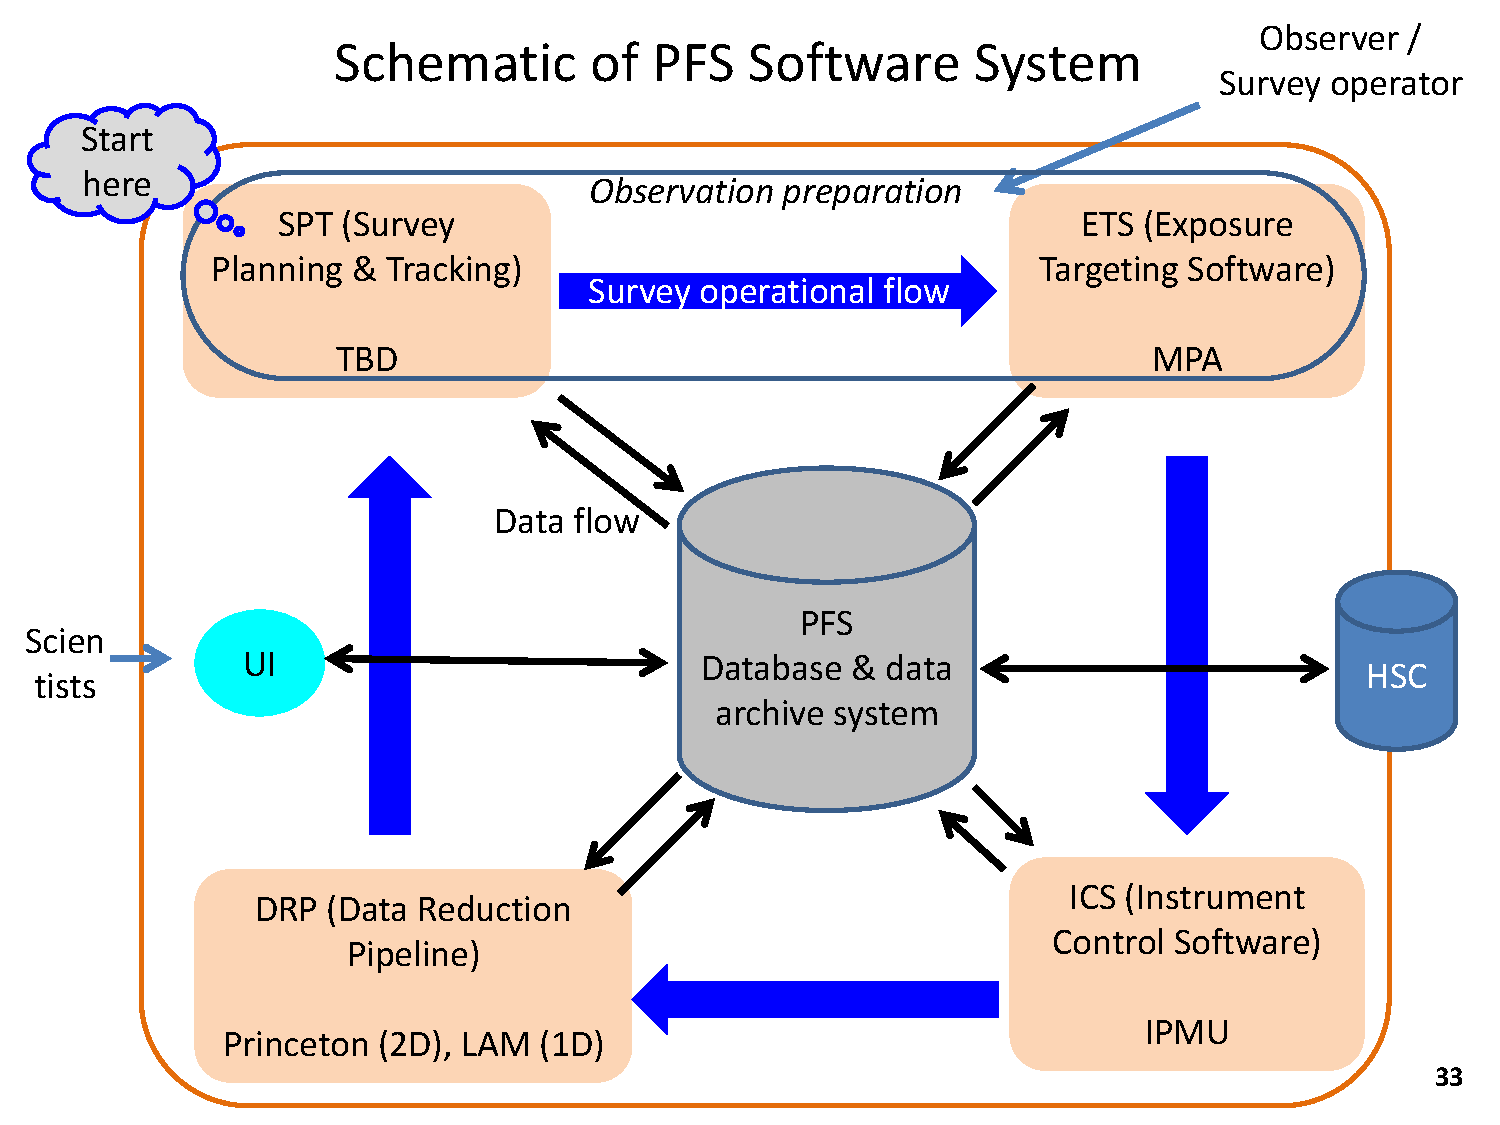
\includegraphics[scale=0.5]{./figures/pfs_survey_operational_concept.pdf}
\end{center}
\caption{A schematic diagram of PFS survey operation concept with the
  four software packages and database/data archive system responsible
  for key processes (to be updated).\label{fig:pfs_survey_concept}}
\end{figure}

For the operation of the PFS instrument and the large survey program
it will carry out, coordination not only between the hardware and
software but also between different software packages is crucial. Four
software components are under development for this, with different
sets of functions packaged and therefore designed to be only loosely
coupled to each other. The detailed definitions of these four packages
have been evolving as the instrument and survey operation concepts are
being updated to maximally accommodate the distinct features of the
planned survey for PFS SSP such as: (1) A much fainter limit than
previous legacy surveys such as SDSS is pursued, exploiting the large
light-gathering power of the Subaru Telescope, (2) given the wide
variety of scientific goals, a wide variety of objects are targeted
for observation and therefore a variety of definitions of success need
to be encompassed, (3)
%successively from FMOS but with a much shorter fiber reconfiguration time,
PFS allows dynamic fiber reallocation even on an individual exposure
basis, unlike the static integration in case of classical multi-slit
and multi-fiber spectroscopy using machined plates. In addition, since
PFS will be a facility instrument at the Subaru Telescope observatory
and will be operated in the framework of general open-use observation,
we are continually discussing all aspects of operations with the
observatory and are trying to adapt our plans accordingly. Below an
overview is given of the current operation concepts and the main
bodies of the software definitions which is sketched out in Figure
\ref{fig:pfs_survey_concept}.
%Technical details are covered in another article\cite{shimono16}.

\subsection{Observation preparation}

The observation process starts with preparing an input target catalog
which includes not only science targets but also stars for field
acquisition, auto-guiding \& focusing, and flux calibration.  Then
telescope pointings, position angles, and fiber allocations to science
targets at each pointing are defined for a given time of observation
(statements about the dot should be here). This planning task is
performed by a software package called {\bf ``ETS'' (Exposure
  Targeting Software)} being developed by Max-Planck-Institut f\"{u}r
Astrophysik (MPA). This observation configuration is prepared by
scientists at sites off the observatory, and the prepared
configuration is then uploaded to a {\bf database} system. At the
actual time of observation, which may be different from the one in the
plan, the details in the mapping between the science targets and
allocated fibers are recalculated before the fiber configuration
starts. Observers should assign a fraction of fibers to observe blank
sky regions and another fraction to observe flux calibration stars
simultaneously with the science targets. The optimal numbers and
distributions of these fibers for sky and calibration targets will be
determined in the course of on-sky engineering observations.

\subsection{Instrument operation \& data acquisition}

\begin{figure}[!htb]
\begin{center}
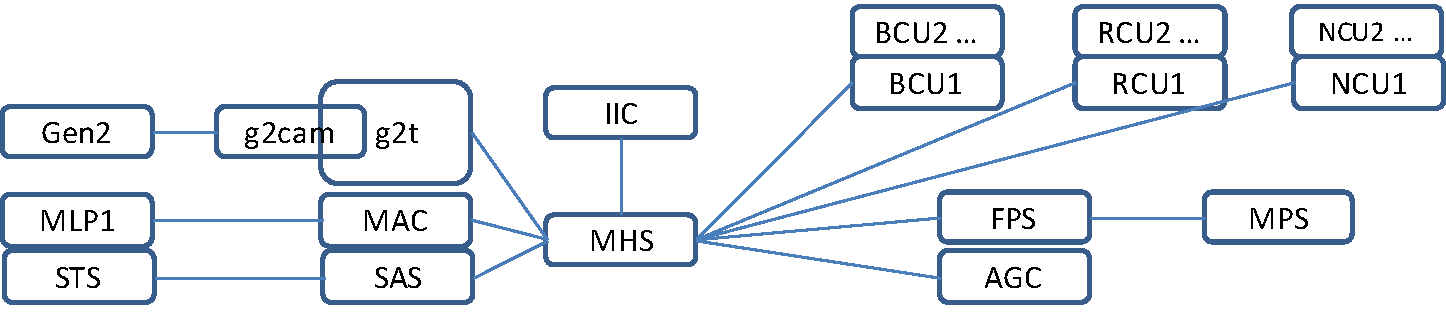
\includegraphics[scale=0.5]{./figures/software_connections.pdf}
\end{center}
\caption{A diagram showing the connections of software components
  around MHS (Messaging Hub System) which is the key to organizing
  distributed processes. \label{fig:pfs_software_connections}}
\end{figure}

{\bf ``ICS'' (Instrument Control Software)} is the software package
that orchestrates the PFS subsystems and subcomponents for instrument
operation in coordination with the telescope system. The key component
for the integration and coordination is a messaging hub system
(MHS). Figure \ref{fig:pfs_software_connections} shows a schematic
diagram of the distributed PFS software components and the telescope
control system connected via MHS. As has been demonstrated in the SDSS
operations at Apache Point Observatory, it efficiently organizes
distributed processes providing uniform communication interfaces
between subcomponents. MHS is being used for the operation of the
CHARIS instrument\cite{charis} (a high contrast integral field
spectrograph for studying disks and extrasolar planets around stars)
which is now in the commissioning phase at the Subaru Telescope, so we
will take advantages of this experience in advance of the PFS
commissioning process.

Details of the telescope and PFS instrument operation will be
explained later in \S~\ref{}, but after various setup processes such
as telescope pointing, instrument rotator rotation, focusing, and
fiber configuration, auto-guiding starts and the spectrograph system
starts taking exposures. The data format from each exposure are two 4K
$\times$ 2K CCDs from the blue and red cameras, and one 4K $\times$ 4K
H4RG detector from the NIR camera. At the end of each exposure, the
data are read out and passed on to the Data Reduction Pipeline (DRP)
for on-site data reduction, data quality assessment \& assurance, and
data archival.

\subsection{Data reduction \& spectral calibration strategy}
\label{subsec:reduction-calibration}

{\bf ``DRP'' (Data Reduction Pipeline)} comprises the ``2D'' part
(2D-DRP) and the ``1D'' part (1D-DRP). The 2D-DRP, which is under
development by PU, receives two-dimensional raw spectral FITS images
read out from the detectors and produces one-dimensional,
sky-subtracted, flux- and wavelength-calibrated spectra ready for
scientific analyses. The 1D-DRP being developed by LAM then receives
these 1D spectra and measures various parameters of spectroscopic
features such as redshifts and emission line fluxes. After each
exposure of the spectrograph detectors, the data will be processed by
on-site DRP with calibration data sets taken in advance.
%checked e.g. by look at the singal-to-noise ratios of bright stars
%such as flux calibration stars and is uploaded to the database.
1D-DRP is applied to the reduced and calibrated 1D spectra and
measured parameters are added to the database. As successive exposures
are taken for the same objects at different nights and observation
runs, deeper and higher quality spectra will be produced from from
full, batch processing of all available data.

One important challenge for this project is to achieve the goal of sky
subtraction accuracy (down to $\sim$0.5\% in the faint sky continuum
between the lines). This means, given that we are not doing
beam-switching operations, that the sky spectrum of an object fiber
needs to be accurately modeled from the spectra of other fibers
looking at the sky, and for this, the two-dimensional fiber PSF needs
to be well characterized as functions of x and y on the detectors
(corresponding to fibers and wavelengths approximately). In other
words, the conditions during the calibration data acquisition need to
closely mimic the observing conditions at night. We have the following
plans for this:

\begin{itemize}
\item We have a calibration lamp system on top of PFI for both
  flat-fielding and wavelength calibration. This lamp illuminates a
  quasi-Lambertian (TBC) screen on the ceiling of the telescope
  enclosure and the illumination reflects back to the telescope
  primary mirror. In this way, the telescope pupil can be diffusely
  illuminated for calibration mimicking the illumination by the sky in
  real observations at night.
\item Even if the pupil illumination is managed as above, differences
  of the fiber status between observations and calibration may cause
  some errors in the PSF modeling due to e.g. variation of Focal
  Ratio Degradation (FRD) in the fibers. There are three cases where
  such errors may be introduced: (1) Fiber moves (mainly twists) as
  the Cobras move, (2) coils/uncoils of fiber bundles with the
  rotation of the instrument by the rotator, and (3)
  bending/unbending of the fiber cable due to telescope elevation
  changes. We currently think that (1) has the most significant
  impact, so the procedure is likely to take the calibration data for
  every fiber configuration taken in a given night. Detailed studies
  are underway. If (2) is also significant, the rotator angle should
  also be reproduced in this data acquisition but the amount of
  calibration data required could be huge and it may not be realistic
  to take them all during a night. If (2) and/or (3) are significant,
  we will plan to have another calibration lamp system to take data
  in the daytime as functions of telescope elevation and rotator
  angle and characterize the impacts.
\item A significant number of fibers should be assigned as sky fibers
  and should be roughly uniformly distributed over the focal
  plane. The required number is still TBD, and will be clarified in
  commissioning observations.
\end{itemize}

\subsection{Data quality assessment and assurance for long-term survey processing}

The procedure of data quality assessment and assurance (QA) is still
being actively discussed in detail, but we are aiming to accommodate a
data QA on an object-by-object basis: Data quality assessment
procedure and success criteria are set for each object so that, once a
particular object is considered ``done'', the fiber(s) assigned to the
object can be allocated to a different target and be reconfigured
accordingly. Also, discussions of a data QA in a short time scale
(much shorter than one night) are underway, for which ``on-site''
(i.e. at the telescope) quick data reduction is needed in addition to
``off-site'' full reduction. In particular for faint objects, one of
the key processes is full analysis of sky fibers even in the quick
on-site data QA to understand the noise characteristics and
subsequently limiting fluxes as a function of wavelength. The database
is then updated with such information, revisions are applied to the
field definitions and/or fiber configurations accordingly, and
observations are performed using such updated fields and fiber
configurations. This routine is repeated until the survey is
considered ``done''. {\bf ``SPT'' (Survey Planning and Tracking
  software)} is the software package for the survey management
responsible for data QA.

%%%%%%%%%%%
%% Detailed Plan %%
%%%%%%%%%%%
\section{Telescope \& Instrument Operation Details\label{sec:detail_ope_plan}}

Below is a list of processes that are carried out in a typical
observing ``night'', including the evening before and morning after
the night.

\begin{itemize}
\item Instrument exchange
\item Startup of the PFS system
\item Telescope \& instrument pre-check
\item Telescope pointing and field acquisition
\item Start of the telescope and instrument rotator operation in the siderial tracking mode
\item Focusing
\item Fiber (re-)configuration
\item Start of telesecope auto guiding
\item ``Science'' exposures of sky
\item ``Calibration'' exposures of domeflat and arc
\item Shutdown of the PFS system
\end{itemize}

These are processed roughly sequentially in the order they appear, but
some of them run in parallel and there are a set of those that are
repeated e.g. every time when the telescope points to a different
field. In what follows, some details of individual processes are
described with such concurrent and iterative processing into
account. These are also visualized and exemplified in the forms of
flowchart and timing chart in Figures
\ref{fig:operation_sequence_overall1} and \ref{fig:operation_sequence_overall2}.

\begin{figure}[!htb]
\begin{center}
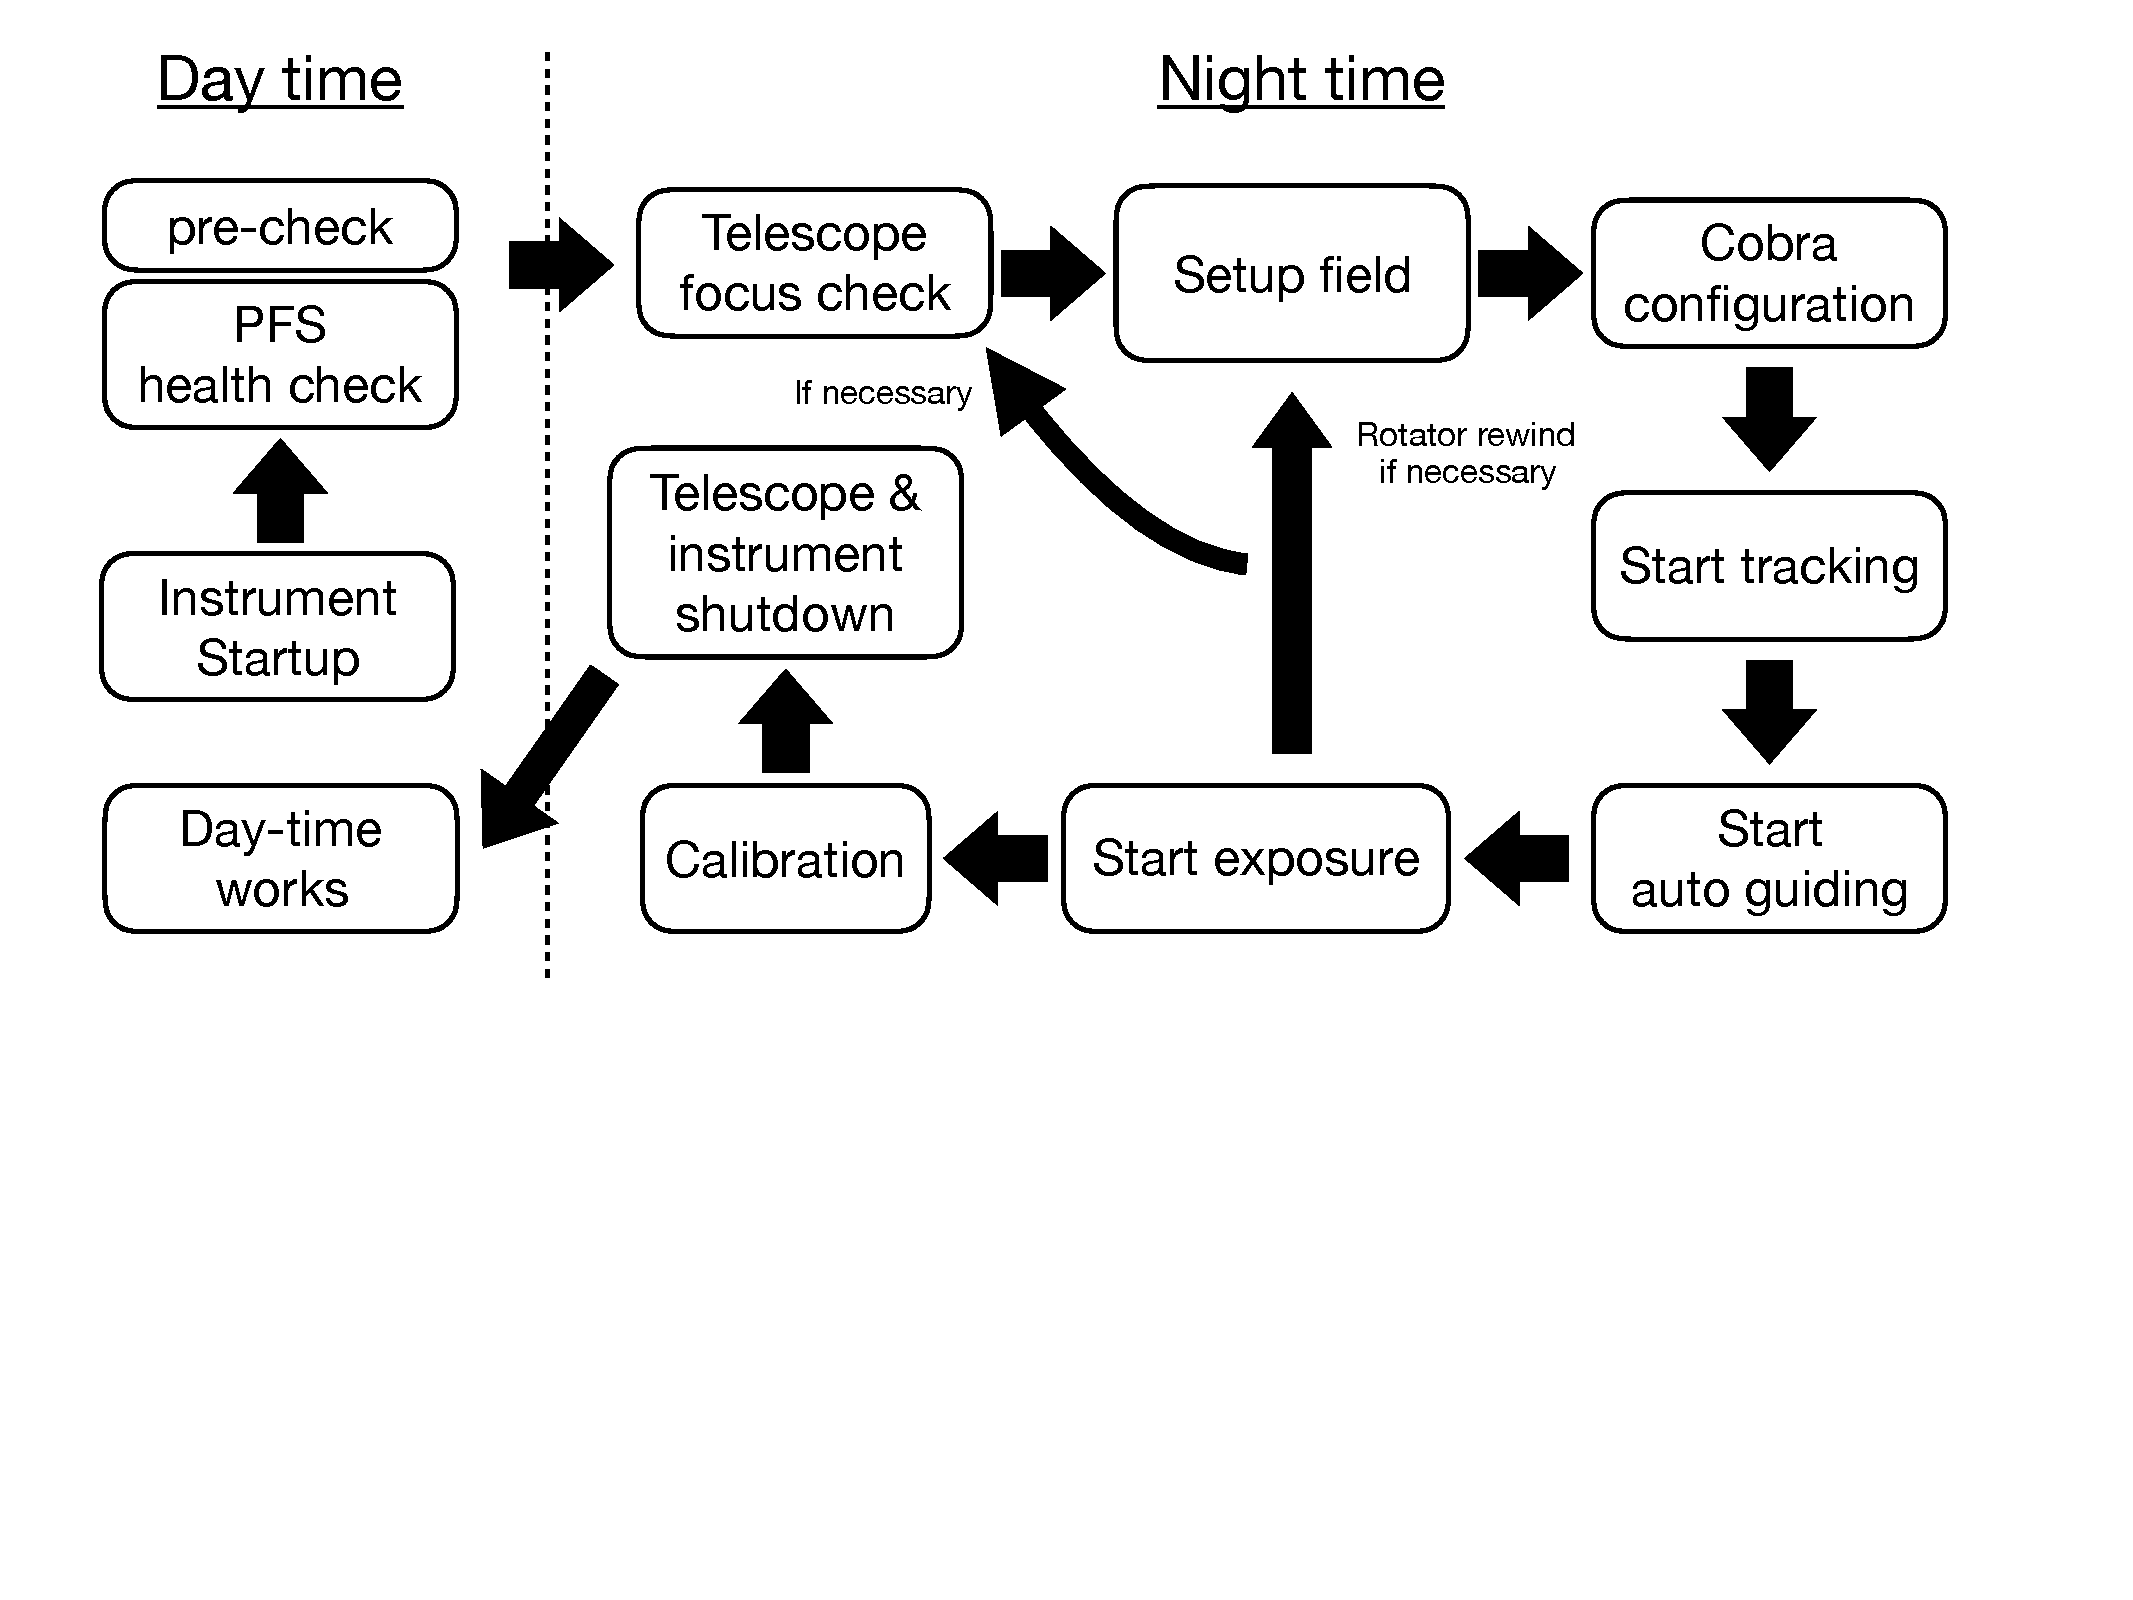
\includegraphics[scale=0.4]{./figures/PFS_night_operation_sequence_overall_cut.pdf}
\end{center}
\caption{An example of the rough operational sequence of the normal scientific observing run. \label{fig:operation_sequence_overall1}}
\end{figure}

\begin{figure}[!htb]
\begin{center}
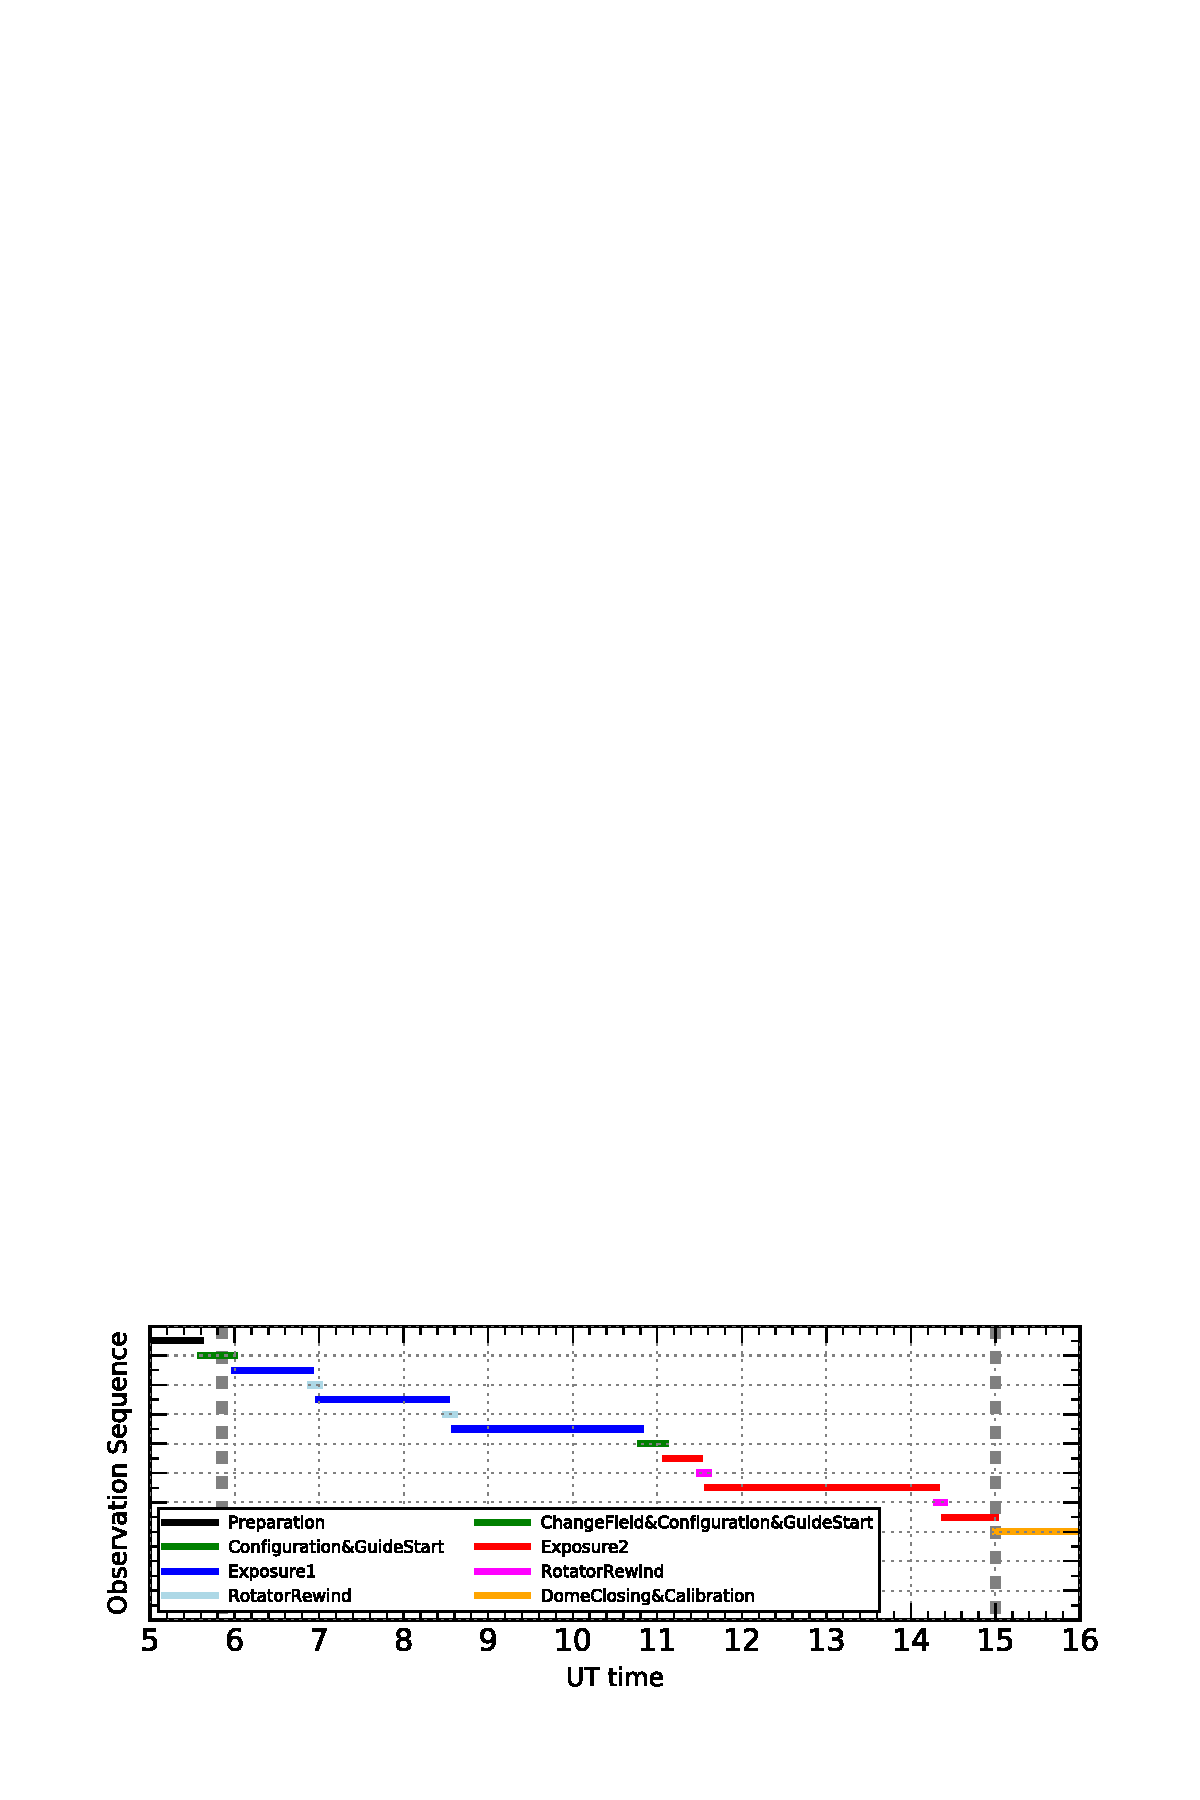
\includegraphics[scale=0.8]{./figures/example_operation_over_night.pdf}
\end{center}
\caption{An example of the time sequence of the normal scientific operation. Here, we assume that moderately long exposures (several hours) are done in two different fields. \label{fig:operation_sequence_overall2}}
\end{figure}

\begin{figure}[!htb]
\begin{center}
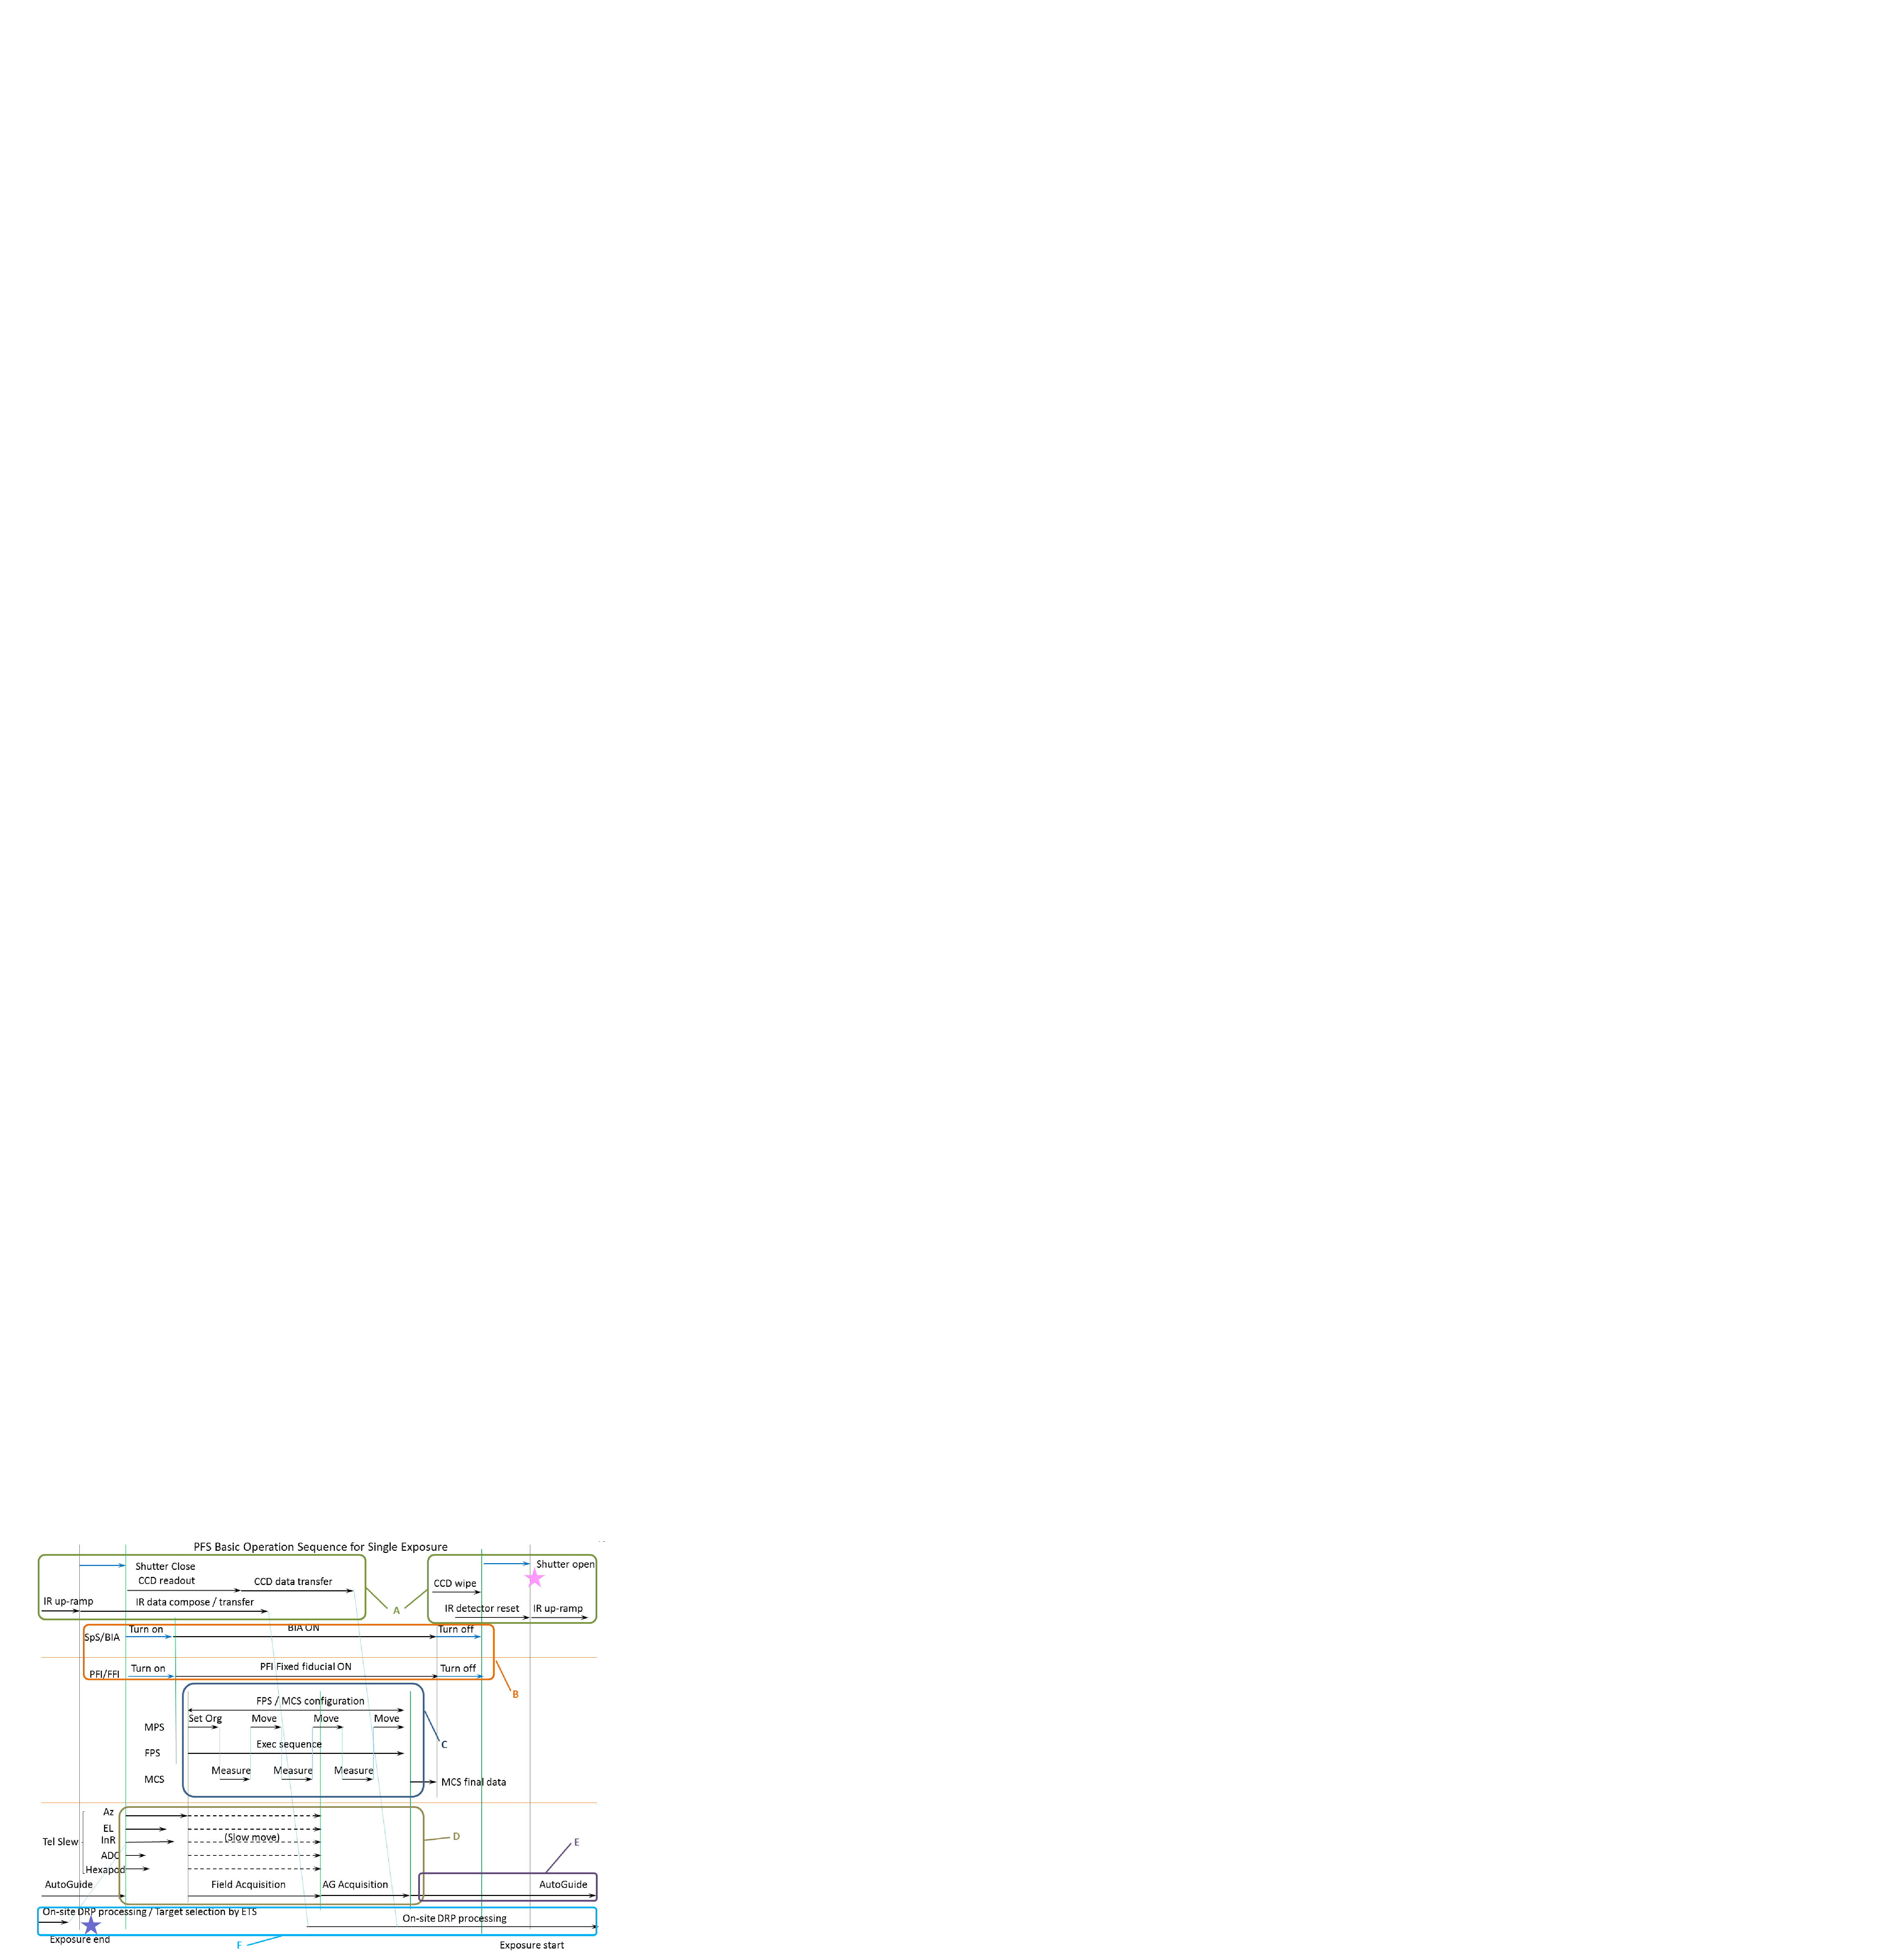
\includegraphics[scale=0.5]{./figures/PFS_Operational_Sequence_for_Single_Exposure_SPIE2016.pdf}
\end{center}
\caption{A schematic view of the operational sequence of instruments as a function of time. (To Be Updated) \label{fig:single_exposure_sequence1}}
\end{figure}

\subsection{Instrument exchange}
In the beginning of the PFS observing runs, the PFS instrument needs
to be set up at the right place on the telescope system. While the
spectrograph system and most of the fiber system are static, PFI and
MCS need to be re-installed every time. Since PFI shares the Popt2
unit with HSC, HSC unit should firstly be removed from the Popt2 if it
is used before the PFS run, and then PFI is installed. MCS is an
assembly as an independent Cassegrain instrument, so it is attached
directly to the Cassegrain port after another Cassegrain instrument is
removed. These installation processes should be described somewhere
else TBD in detail.\\

\subsection{Startup of the PFS system}

The basic procedure of this startup is supposed to be the following.

\begin{itemize}
\item Power ON each sub-system
\item Run an initialization process on each sub-system and confirm its
  operation.
\item Establish the communication between the sub-systems via ICS
\item Leave them in a stand-by/ready state for the next process
\end{itemize}

Note that the spectrograph system is static (i.e. no need of something
like instrument exchange), so it can be left in a ready status for a
long time between PFS runs. Meanwhile, PFI and MCS are reinstalled at
the beginning of every run. So they can be turned on at the stand-by
positions for initialization and test/maintenance processes, but they
are supposed to be turned off before the installation processes and
the startup sequence is applied again after they get on the telescope.

The details of each process in this startup procedure should be
developed and written down with a step-by-step procedure. A
preliminary one will be developed at a sub-system level by the time of
its delivery to the observatory, and it will be further developed by
the collaboration with the observatory staffs in the process of
re-integration and commissioning at Subaru.

\subsection{Telescope \& instrument pre-check}
Once the instrument exchange is completed, the pre-check is performed
before the night operation starts. This pre-check covers the health
and readiness check of not only the telescope system but also the PFS
instrument. The pre-check of PFS should be developed in detail in the
future by collaboration with the observatory staffs, but will likely
be composed of a subset of subsystem check processes and those to
check the system operation on the telescope.

\subsection{Focusing}
There are three foci important for the PFS operation: The prime focus,
MCS focus, and SpS focus. The prime focus is checked by the images of
bright stars on the PFS AG cameras after the sun sets and the dome
opens. There are six AG cameras surrounding the PFS science field of
view where the fibers are populated. In front of each AG camera
sensor, there is a setup by which the half area of camera sensor is
covered by a slightly different optical path length from the other
half, so that by looking at the stellar images and comparing those in
one area with the other, one can determine which way the focus should
be shifted. The focus is adjusted by the Hexapod which can change the
distance from the telescope primary mirror to the assembly of WFC and
PFI. We intend to implement this focus adjustment in parallel to
running field acquisition and auto guiding. Since the focus should
vary during a night, we shoud monitor it and apply correction if
needed. The frequency of the focus check is not clear at this moment,
but we probably need to do a few focus checks during a night. 

Meanwhile, we assume the other two foci will have already been set to
the optimal positions before the evening of a PFS observing night. The
focus position of the detector in MCS will be optimized in the
commissioning phase looking at the back-illuminated fibers at the
prime focus. Opto-mechanically MCS is reasonablly thermalized within a
temparature range typically expected during a night, so we expect only
occasionally to have to adjust the focus position. Note that the image
quality on the MCS detector is quite insensitive to the distance
between the prime focus and MCS as a bulk.

The SpS focus will also be optimized in the integration and
commissioning phase using the hexapod mechanism under the fiber slit
assembly and the detector focus mechanism in each camera. This process
can be done independent of the status of the other PFS subsystems and
the telescope using the internal illumination source of SpS. Since SpS
is locaetd in the temperature-controlled Spectrograph Clean Room
(SCR), once the focus is optimized, we expect only occasionally to
have to check and adjust it again. One exception may be when the
configuration of the red camera is changed to the medium-resolution
mode from the low-resolution mode or vice versa in the middle of a
night: Although the spectrograph has been designed in such a way that
no focus adjustment is needed between these two setups with different
gratings, we will have to confirm this in the commissioning phase.

\subsection{Telescope pointing and field acquisition}
The first step in actual observations is to point the telescope to the
target field and set the instrument rotator to a requested angle.  In
parallel, the Hexapod, ADC, and telescope primary mirror active
support are adjusted by the telescope control system for this new
field. Once the telescope and rotator stop slewing and start operating
in the tracking mode, exposures of acquisition stars are taken by the
AG cameras, errors in the telescope pointing and rotator angle are
calculated, and feedback is sent to the telescope control system for
corrections.  This process is iterated continuously until the errors
are small enough to start auto-guiding. A focusing operation can be
executed at some point in this course of field acquisition and
auto-guiding.

\subsection{Fiber (re-)configuration}
While the telescope is slewing, the fiber positioner system can start
configuring the science fibers at least coarsely to the expected
positions of the science targets on the focal plane. When the process
of fiber configuration starts, SpS closes the shutters and starts
reading out the detectors. It also turns on the LEDs to illuminate the
surfaces of the shutters (the other sides from the cameras are
illuminated, so there is no interference to the detector
readouts). The diffuse reflection of the LED lights illuminates the
collimator mirror and is focused by the collimator mirror back onto
the fiber slit. In this way, the fiber tips at the prime focus are
back-illuminated. Meanwhile, the fixed fiducial fibers are illuminated
by the fiducial illuminator accommodated in PFI. MCS then takes images
of the back-lit science and fiducial fibers, measures the current
positions of them and calculate the errors from the requested
positions of the science fibers. Based on this information the fiber
positions are updated and the errors get smaller as successive
iterations are applied. Once the telescope and rotator start operating
in the siderial tracking mode, the rotator operation and auto-guiding
are temporarily stopped\footnote{When observations are carried out
  using the prime focus, the prime focus instrument can be rotated,
  but the Cassegrain instrument cannot be operated because the focus
  is not in use. Accordingly, the MCS cannot be rotated synchronously
  with PFI and therefore the images of back-illuminated fibers on MCS
  are elongated if PFI is rotated and could worsen the centroiding
  error.}  for fine positioning of the fibers (the telescope can still
be moving in the tracking mode).
%
Apart from the time for telescope slewing and rotator operation, one
iteration of fiber configuration is expected to take $\sim$10$-$15sec,
including both the time of Cobra moves and exposure time of MCS. We
expect $\sim$6 iterations will be required, so one fiber
configuration will be completed in $\sim$90sec given several
iterations are needed, but more studies are on-going to fully
understand the timing budget.

\begin{figure}
  \begin{center}
    \begin{tabular}{ccc} %% tabular useful for creating an array of images
      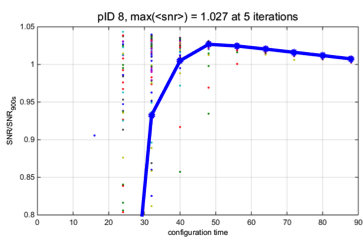
\includegraphics[width=7.5cm]{./figures/cobra-sn.png} &
      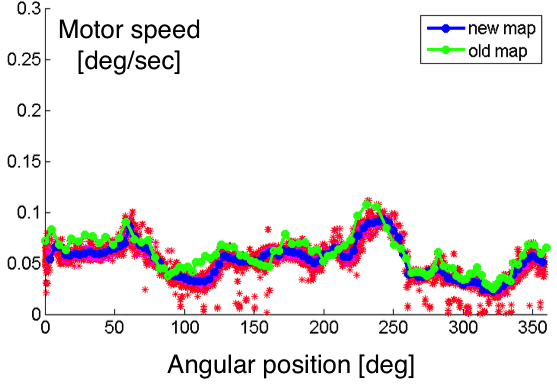
\includegraphics[width=7.5cm]{./figures/cobra-motormap.png} \\
    \end{tabular}
  \end{center}
  \caption{ \label{fig:cobraperformance} On the left, the level of
    convergence of Cobras to requested positions is plotted against
    measure of the signal-to-noise ratio relative to a fiducial value,
    which increases to the maximum at the fourth iterations and slowly
    decreases at later iterations. These data were taken at the target
    convergence tests on the engineering model Cobra positioners
    module. On the right, the data points indicate the Cobra motor
    speeds as a function of angular position. The relationship is
    so-called a motor map. As two curves are shown in the graph, a
    motor map can be updated as more data are collected.}
\end{figure}

Below are a few details to be highlighted in the procedure of
observation and data acquisition procedure:

\begin{itemize}
\item It is not trivial to determine that the Cobras are aligned well
  enough to the target positions. Actual criteria for convergence and
  procedure of assessment are still under discussions, but we
  consider that the concept of a signal-to-noise ratio can be useful
  as a measure of optimality, rather than the residual distances of
  the fibers from their targets. Starting from a situation in which
  all the fibers are remote from their target positions (except for
  chance coincidence), in the first few iterations, all the fibers get
  closer to the targets, so the signal in terms of fluxes from the
  objects to the fibers increases quickly. However, the gain of the
  signal after each move of the Cobras gets smaller at later
  iterations because most of the fibers are already reasonably close
  to the targets, and then the gain becomes less than the loss due to
  the loss of the observing time for integration on the
  detectors. Therefore the number of iterations giving the optimal
  signal-to-noise ratio must be somewhere in the middle
  (Fig. \ref{fig:cobraperformance}). In reality, since the time for
  one iteration is rather short in particular at later iterations,
  some more iterations to pursue better positions of more fibers may
  be worth at relatively small expenses of observing time, so we will
  leave such flexibility in the choice.
\item The response of each motor in the Cobra actuator to a drive
  signal is known to depend on angular position
  (Fig. \ref{fig:cobraperformance}). Characterizing this so-called
  ``motor map'' and operating the Cobras taking it into account are
  considered key to achieve efficient convergence.
\item Although observation strategies and data quality success
  criteria are different among the three main science areas in the
  plan of PFS SSP survey\cite{takada14}, all are planning to acquire
  data with no beam-switching to blank sky. (The instrument control
  system will however accommodate the beam switching capability as an
  option.)  This will maximize the on-source integration time over the
  observing time and minimize the geometric constraints in the
  allocation of science fibers to science targets\footnote{In
    cross-beam switching observations, two fibers are assigned to one
    science target and the telescope pointing is dithered between one
    exposure and another so that in the first exposure one of the
    fibers is placed on the target and the other observes blank sky,
    and in the next exposure, they switch the role. This way, 100\% of
    the exposure time can be used for on-source integration, but the
    fibers can be significantly less flexibly allocated to targets.}.
 \item Due to the large field of view, the differential atmospheric
   refraction effect is severe over most of the sky. Accordingly, the
   science fibers need to be reconfigured e.g. every $\sim$30 minutes
   (TBC).
%\item The instrument rotator operates over a restricted range between
%  $-60$ deg to $+60$ deg. This is to minimize any variation of the
%  fiber status by instrument rotation (possibly important for stable
%  Point Spread Function (PSF) on the spectrograph detectors and
%  therefore for good sky subtraction), exploiting the hexagonal
%  symmetry on the PFS focal plane.
\end{itemize}

\subsection{Start of telescope auto guiding and ``science'' exposures}

Once the fiber configuration is complete, the rotator operation is
restarted, the field acquisition process is redone and the
auto-guiding operation is restarted. In parallel, SpS turns off the
LEDs for science fiber back-illumination and PFI turns off the
fiducial illuminator. Then SpS opens the shutters and starts exposing
the detectors to the sky.

\subsection{When should the fibers be reconfigured?}

In most cases of the PFS survey observation, multiple exposures for
the same targets and fiber configuration are expected, but we should
likely repeat exposures with often updating the fiber configuration.
There are a few reasons for this:

\begin{itemize}
\item Due to the large field of view, the differential atmospheric
  refraction effect is severe over most of the sky. Accordingly, the
  science fibers need to be reconfigured e.g. every $\sim$30 minutes
  (TBC).
\item In the current plan, the data quality assessment and assurance
  are carried out on an individual object basis. So, even if the same
  area of sky is integrated, the fiber configuration should partially
  change from exposure to exposure as integrated data of some targets
  show e.g. high enough signal-to-noise ratio.
\end{itemize}

\subsection{Rewinding the instrument rotator}

In the PFS operation, the range of instrument rotator angle is
intentionally restricted by the software to that from $-60$ deg to
$+60$ deg (mechanically it can rotate from $-270$ deg to $+270$ deg
with no damage to the instrument). This is to minimize any variation
of the fiber status by instrument rotation (possibly important for
stable Point Spread Function (PSF) on the spectrograph detectors and
therefore for good sky subtraction), exploiting the hexagonal symmetry
on the PFS focal plane. This means that we need to rewind the rotator
by 60 or 120 deg when the rotator angle hits the limit (see
\ref{appendix:documents:yabe}). Figure
\ref{fig:operation_sequence_overall2} shows an example of the
operation over night for a case that observations with multiple
exposures in two different fields. In this case, we need to rewind the
rotator two times in each field.

\subsection{Calibration exposures}

In the current plan, calibration exposures (i.e. domeflat frames and
arc frames) are taken only at the beginning and end of a night
(i.e. in the evening and morning) when the dome is closed and the
telescope points to the zenith. The PFS instrument is equipped with
its own calibration lamp system on top of PFI for flat-fielding and
wavelength calibration. These lamps will be turned on, and exposures
are taken. The mirror cover should be left open in this data
acquisition for the light come into the instrument as similarly as
possible to the case of observing the sky. Also, to reproduce the
fiber status in the observing conditions as much as possible, we
consider to configure the science fibers in the same way as observing
the sky. We believe fine positioning is not needed, so a small number
of iterative moves should be enough for the fiber configuration.
However, if science exposures are taken with different fiber
configurasions during a night, subsequently a set of calibration
frames for each configuration need to be taken as in the case of FMOS
calibration data acquisition. As mentioned in
\S~\ref{subsec:reduction-calibration}, if we find additinal variation
for some reasons with the telescope elevation angle, time,
environmental conditions, and so on, we may need to take calibration
exposures more frequently. We will clarify needs in the engineering
observations.

\subsection{Shutdown of the PFS system}

This process is to terminate the PFS operation. Overall there are two
cases: One is when a PFS observing run finishes (so this shutdown is
done at the last morning before instrument exchange where PFS is
removed from the telescope), and the other is when one night of PFS
observation finishes but the run still continues (i.e. PFS observation
is scheduled also on the next night). In the latter case, the
instrument should be turned into a stand-by or sleep mode (to be
defined, though) rather than shutdown completely so that it can be
restarted efficiently at the beginning of next night.

The shutdown sequence is supposed to be roughly as follows, although
many details should be developed through the collaboration with the
observatory staffs.

\begin{itemize}
\item Stop the current procedure (probably calibration mode?) normally
\item Check the system is in the safe state for shutdown process
\item Turn the power systems OFF (especially PFI and MCS for removal from the telescope)
\end{itemize}

After the shutdown procedure is done, PFI and MCS should become ready
for removal from the telescope in the day time.

As described in \ref{sec:survey_operation:software}, the entire instrument operation is done with sequences associated with each instrumental component. Here we described the detailed processes of each sequence and their relation between each other.

%%%%%%%%%%%%%%%%%%%%%%%%%%%
%% Operational sequence during engineering  %%
%%%%%%%%%%%%%%%%%%%%%%%%%%%
\subsection{Special operations for commissioning, engineering, maintenance purposes\label{sec:detail_ope_plan:engineering}}

Operation details are to be written for individual processes like
below needed in the commissioning phase.

\begin{itemize}
\item The xy and tilt alignment of the assembly of WFC and PFI against
  the telescope primary mirror by using defocused images of a bright
  star on the AG cameras
\item Measuring the rotator center position relative to PFI focal plane using MCS
\item Detailed characterization of PSF on the spectrograph detectors
  by masking quite a few fibers under the Field Element dots and making a sparse distribution of spectra on the detectors
\item Initial characterization of Cobras: Arm lengths, phi and theta axes, etc.
\item First-pass distortion map using the AG camera images
\item Raster scan for 2nd-pass distortion map and its fine tunes
\item Making formulae of relative flux calibration from observation of bright $\sim$F stars

\end{itemize}

%%%%%%%%%%%%%%%%%%
%% Connection with Tel system %%
%%%%%%%%%%%%%%%%%%
\section{Implementation plan (pretty much under development)}
\subsection{Connection between PFS and the telescope systems}
The coordination of the telescope and the instruments at the summit is
done by Gen2 system. In the operation of PFS system in the normal
observing mode, ICS is required to communicate with Gen2 to receive
the telescope status and also send the status of the instrument and
requests for the movement to the telescope. The communication between
the PFS system (MHS) and the telescope (Gen2) is done via an interface
called ``g2t'' by using ``g2cam'' library in Python.

As we mentioned in section \ref{sec:detail_ope_plan:overall}, each
sub-sequence can be processed in parallel. Since any commands in g2cam
can be triggered only by Gen2, the sequence should be done in the
following way:
\begin{itemize}
\item Gen2 prepares a command for callback
\item Once the event occurs, PFS pushes the status with what should be done by Gen2 (such as rotate InR by 120 deg.) and ends the command
\item The sequence running in Gen2 picks up the status value and execute the command
\item Return to the 1st step (if necessary)
\end{itemize}
The detailed processing during the single exposure is described in the section \ref{sec:detail_ope_plan:single}.

Another interface is between the status server called Subaru Telemetry
System (STS) and the PFS internal Status Archival System
(SAS). Various information on the instrument status is stored in SAS
and some of them should also be stored in STS.

\begin{figure}[!htb]
\begin{center}
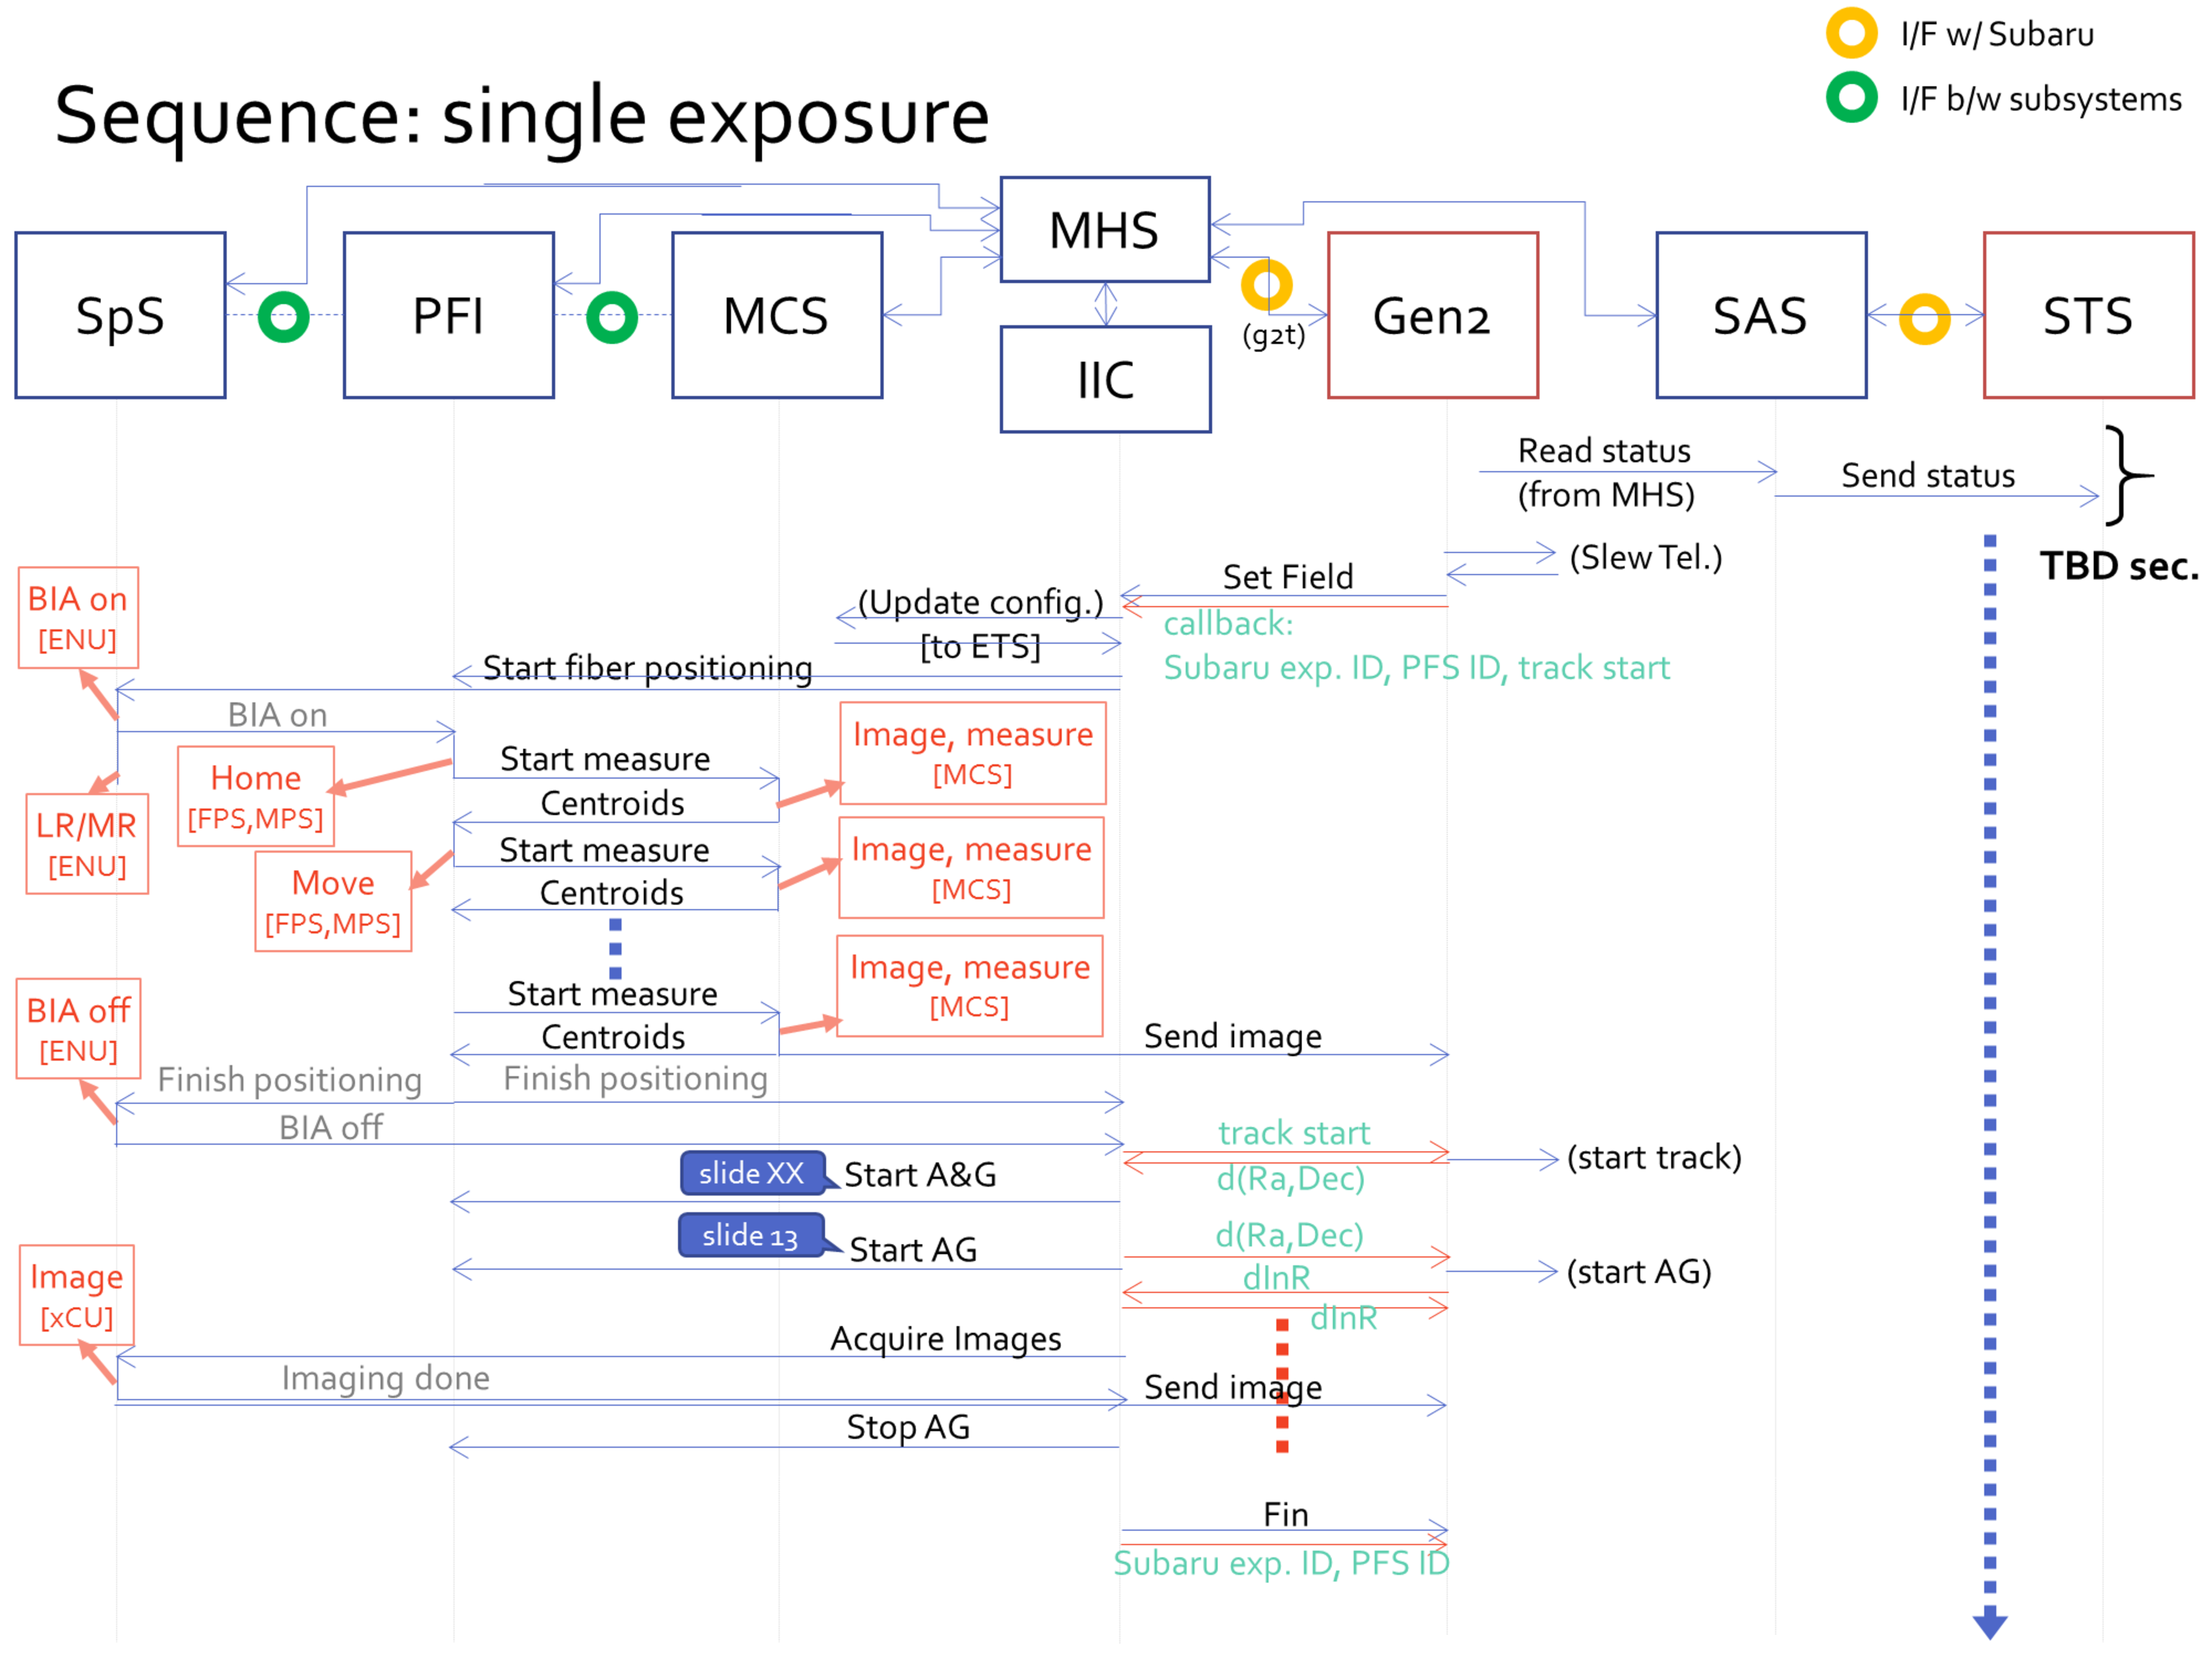
\includegraphics[scale=0.2]{./figures/PFS_sequence_process.pdf}
\end{center}
\caption{A schematic view of the communication between each sub-component during the operation. (To Be Updated)\label{fig:single_exposure_sequence2}}
\end{figure}

%%%%%%
%% QA %%
%%%%%%
\subsection{Checking the quality of the obtained data}
%%%%%%%%%%
%% Summit QA %%
%%%%%%%%%%
\subsubsection{Summit QA of the obtained data (inputs from Robert Lupton?)}
\noindent \underline{\textbf{Initial check of the obtained data:}}
\vspace{5pt}

A monitoring system of the obtained 2D images whether it is a scientific data or not would be helpful for the initial check of the obtained data. This is also useful for the health check of the instrument. The following items should be included in the monitoring system:\\

\begin{itemize}
\item A FITS viewer of the obtained 2D images
\item Measurement of the count level at a given position on the image
\item Zoom-in function for detailed inspections
\item Scale and contrast change for detailed inspections
\end{itemize}

Some functions are already implemented on the current Gen2 system.\\

\noindent \underline{\textbf{Autoguiding monitoring:}}
\vspace{5pt}

The variation of the positional accuracy of assigned fibers to objects
is critical to the signal-to-noise ratio of the obtained spectra. The
statistical positional errors of the fibers is monitored by the
centroids of bright stars in the A/G cameras. Again, bright (point
source-like) galaxies can be used for this purpose. Not only the
statistics but also a monitoring system with GUI may be useful to
observers.\\

\noindent \underline{\textbf{Sky condition monitoring:}}
\vspace{5pt}

The weather condition including seeing and transparency at a given
time during the observation is essential to the precise measurements
of fluxes of the obtained spectra. Bright stars in the A/G cameras are
used for the monitoring of the weather condition. If we have too few
stars in the FoVs of the A/G cameras, we alternatively use bright
galaxies (as point source-like as possible) for these purposes. FWHM
of the object image at a given time is at lease required to quantify
the seeing size. The difference between the obtained fluxes and the
catalogue values is used for the monitoring the sky
transparency. Here, we expect precise photometry in HSC or SDSS and
other catalogues.

Another possibility to monitor the sky condition during the night is
to measure the flux level of the obtained spectra of e.g. standard
stars in each arm. In particular, monitoring the continuum level of
blue arm gives us information on the effect of the moon light, and the
flux level of the red and/or NIR arm could be useful to the variation
of OH sky lines. At least an interface to show the summary of the
quality of the obtained spectra is desirable on the summit system
(TBD).\\

%%%%%%%%%%
%% Off-site QA %%
%%%%%%%%%%
\subsubsection{Off-site QA of the obtained data (also inputs from Robert Lupton?)}
TBW

%%%%%%%%%%%%%
%% Queue operation %%
%%%%%%%%%%%%%
\subsection{PFS operation in queue mode}
TBW 

%%%%%%%%%%%
%% Possible trouble %
%%%%%%%%%%%
\section{Possible troubles during the operation and tips for them}
In this section, we describe possible troubles envisioned and the
solutions during the operation.
\subsection{Possible troubles in general}
\subsection{Possible troubles during the system startup/shutdown, the pre-check, and the instrument health check}
\subsection{Possible troubles during the scientific operation}
\subsection{Possible troubles during the calibration operation}

\begin{thebibliography}{99}
\bibitem{tamura16} Tamura, N., et al., ``Prime Focus Spectrograph (PFS) for the Subaru telescope: overview, recent progress, and future perspectives'', Proc. SPIE 9908, Ground-based and Airborne Instrumentation for Astronomy VI, 99081M (9 August 2016); doi: 10.1117/12.2232103
\bibitem{wang16pfi} Wang, S., et al., ``The current status of prime focus instrument of Subaru prime focus spectrograph'', Proc. SPIE AS105PS, Ground-based and Airborne Instrumentation for Astronomy VI Posters, 990882 (9 August 2016); doi: 10.1117/12.2232044
\bibitem{takato14} Takato, N., et al., ``Design and performance of a F/\verb|#|-conversion microlens for prime focus spectrograph at Subaru Telescope'', Proc. SPIE 9147, Ground-based and Airborne Instrumentation for Astronomy V, 914765 (31 July 2014); doi: 10.1117/12.2055051
\bibitem{fisher14} Fisher, C., et al., ``Developing engineering model Cobra fiber positioners for the Subaru Telescope’s prime focus spectrometer'', Proc. SPIE 9151, Advances in Optical and Mechanical Technologies for Telescopes and Instrumentation, 91511Y (7 August 2014); doi: 10.1117/12.2054700
\bibitem{wang16mcs} Wang, S.. et al., ``Metrology camera system of prime focus spectrograph for Suburu telescope'', Proc. SPIE AS105PS, Ground-based and Airborne Instrumentation for Astronomy VI Posters, 990881 (9 August 2016); doi: 10.1117/12.2232035
\bibitem{madec16} Madec, F., et al., ``SUBARU prime focus spectrograph: integration, testing and performance for the first spectrograph'', Proc. SPIE AS105PS, Ground-based and Airborne Instrumentation for Astronomy VI Posters, 99088U (9 August 2016); doi: 10.1117/12.2233057
\bibitem{gunn16} Gunn, J. E., et al., ``Detector and control system design and performance for the SuMIRe prime focus spectrograph (PFS) cameras'', Proc. SPIE AS105PS, Ground-based and Airborne Instrumentation for Astronomy VI Posters, 990893 (9 August 2016); doi: 10.1117/12.2233400
\bibitem{smee16} Smee, S. A., et al., ``Visible camera cryostat design and performance for the SuMIRe Prime Focus Spectrograph (PFS)'', Proc. SPIE AS105PS, Ground-based and Airborne Instrumentation for Astronomy VI Posters, 99088Y (9 August 2016); doi: 10.1117/12.2233185
\bibitem{hart16} Hart, M., et al., ``A novel reflectometer for relative reflectance measurements of CCDs'', Proc. SPIE 9915, High Energy, Optical, and Infrared Detectors for Astronomy VII, 99152D (27 July 2016); doi: 10.1117/12.2232943
\bibitem{cesar16} de Oliveira, A. C., et al., ``Fiber optical cable and connector system (FOCCoS) for PFS/ Subaru'', Proc. SPIE 9151, Advances in Optical and Mechanical Technologies for Telescopes and Instrumentation, 91514G (28 July 2014); doi: 10.1117/12.2056888
\bibitem{charis} Groff, T., et al., ``Laboratory testing and performance verification of the CHARIS integral field spectrograph'', Proc. SPIE 9908, Ground-based and Airborne Instrumentation for Astronomy VI, 99080O (9 August 2016); doi: 10.1117/12.2233447
\bibitem{takada14} Takada, M., et al., ``Extragalactic science, cosmology, and Galactic archaeology with the Subaru Prime Focus Spectrograph'', Publications of the Astronomical Society of Japan, Volume 66, Issue 1, id.R1 (2014)
\end{thebibliography}

\clearpage
\appendix
%%%%%%%%%%%%%%%%
%% Pointers to documents %%
%%%%%%%%%%%%%%%%
\section{Pointers to technical documents}

\subsection{Documents by Atsushi Shimono \label{appendix:documents:shimono}}
\begin{itemize}
\item \href{http://sumire.pbworks.com/w/file/102897967/SSN-00011-001-ICSSeq-1-Overall.pptx}{SSN-00011-001} (Study on PFS Observation Sequence (I) Overall)
\item \href{http://sumire.pbworks.com/w/file/94687160/SSN-00012-001-ICSSeq-2-CommandToAG.pptx}{SSN-00012-001} (Study on PFS Observation Sequence (II) From command next field to AutoGuide)
\item \href{http://sumire.pbworks.com/w/file/93138234/SSN-00006-001-AGtoGen2.pptx}{SSN-00006-002} (Study on PFS A\&G/AG communication)
\item \href{http://sumire.pbworks.com/w/file/101124121/SSN-00016-001-Gen2-OBCP.pptx}{SSN-00016-001} (Connection from PFS ICS to Gen2)
\item 
\end{itemize}

\subsection{Documents related to the commissioning by Yuki Moritani\label{appendix:documents:moritani}}
\begin{itemize}
\item \href{}{PFS commissioning plan}
\end{itemize}

\subsection{Documents related to various studies on PFS operation by Kiyoto Yabe\label{appendix:documents:yabe}}
\begin{itemize}
\item \href{http://member.ipmu.jp/kiyoto.yabe/PFS/tmp/material_pfs_operation_dots_20160629.pdf}{material\_pfs\_operation\_dots\_20160629.pdf} (Effects of instrument rotator angle on dot coverage on the focal plane)
\end{itemize}

%%%%%%%%%%%%%%
%% Operation of FMOS %%
%%%%%%%%%%%%%%
\section{The operational process in FMOS}
\subsection{}


\end{document}
